\documentclass[a4paper,12pt]{article}
\usepackage[danish]{babel}
\usepackage[utf8]{inputenc} %laver æ ø og å
\usepackage{lmodern}
\usepackage[T1]{fontenc}
\usepackage{amsmath}
\usepackage{graphicx}
\newcommand{\vect}[1]{\boldsymbol{#1}}
\usepackage{amsfonts}
\usepackage{amssymb}
\usepackage{ dsfont }
\usepackage{mathtools}
\DeclarePairedDelimiter\abs{\lvert}{\rvert}
\DeclarePairedDelimiter\norm{\lVert}{\rVert}
\usepackage{mathrsfs}
\usepackage{ stmaryrd }
\usepackage[parfill]{parskip}
\usepackage{fancyhdr}
\pagestyle{fancy}
\usepackage{lastpage}
\usepackage{placeins} %til billeder
\usepackage{enumitem}
\usepackage{listings}
\documentclass{article}
\usepackage{resizegather}
\usepackage{xcolor}
\usepackage{bbm}
\usepackage{booktabs}
\usepackage{array}
\usepackage{hyperref}
\usepackage{pbox}
\usepackage{listings}
\usepackage{mcode}
\usepackage{siunitx}
\usepackage[romanian]{babel}
\usepackage{combelow}
\documentclass{article}
\newcommand\barbelow[1]{\stackunder[1.2pt]{$#1$}{\rule{.8ex}{.075ex}}}
\usepackage{subcaption}
\usepackage{stackengine}
\usepackage{amsthm}
\newcommand\independent{\protect\mathpalette{\protect\independenT}{\perp}}
\def\independenT#1#2{\mathrel{\rlap{$#1#2$}\mkern2mu{#1#2}}}
\makeatletter
\newcommand*\bigcdot{\mathpalette\bigcdot@{.5}}
\newcommand*\bigcdot@[2]{\mathbin{\vcenter{\hbox{\scalebox{#2}{$\m@th#1\bullet$}}}}}
\makeatother

\graphicspath{ {images/} }
\date{}
\fancyhf{}
\cfoot{Page \thepage\ of \pageref{LastPage}}
\renewcommand{\headrulewidth}{0pt}
\renewcommand{\footrulewidth}{0pt}
\title{Diffusions and stochastic differential equations - Report 2}
\author{\\\mbox{} \\Name: Jonathan Kiersch, \mbox{} \\ Student-ID: s144252 }
\setcounter{section}{0}
\documentclass{article}

\newtheorem{definition}{Definition}
\newtheorem{theorem}{Sætning}
\newtheorem{corollary}{Korollar}
\newtheorem{note}{Bemærk}
\newcommand{\mat}[1]{#1}
\newcommand{\vect}[1]{#1}

\begin{document}

\maketitle
\thispagestyle{fancy}

\section{Introduction}



\section{Question 1 - A stochastic predator-prey model}

We are considering a coupled system of stochastic differential equations who are governing a model for predator and prey dynamics in a given environment. The size of the prey population is modelled by the It\^{o}-process $\{N_t\}$ and $\{P_t\}$ models the predator population. The It\^{o} equation for the joint proces $(N_t, P_t)$ is given by the following\\

\begin{equation}
\begin{aligned}
\label{ex11}
dN_t&= rN_t(1-N_t/K)\cdot dt-\beta N_tP_t\cdot dt +\sigma_N N_t \cdot dB_t^{(1)}\\
dP_t&= \epsilon \beta N_t P_t\cdot dt-\mu P_t\cdot dt +\sigma_P P_t \cdot dB_t^{(2)}\\
\end{aligned}
\end{equation}

where $\{B_t^{(1)}\}$ and $\{B_t^{(2)}\}$ are two independent standard Brownian motion and the model parameters $r, K, \beta, \epsilon, \sigma_N, \sigma_P$ are all positive. Furthermore and naturally, we only accept $N_t\geq 0$ and $P_t\geq 0$, because it would make litte sense to look negative population sizes.\\

\subsection{Task 1 - Simulation}


Now we want to simulate the model in eq.(~\ref{ex11}) with fixed parameters $r=1, K=1, \beta=10, \epsilon=0.1, \mu= 0.05, \sigma_N=0.1, \sigma_P=0.1$ and initial conditions $N_0=P_0=10^{-4}$.\\

We first choose to simulate the system with a simple Euler-Maruyama method, which we apply directly on the system. Thereafter, we try to convert the above It\^{o} system into a Stratonovich system and apply Heun's method on it, as we remember from Assignment 1, the Heun method was clearly better on our SDE system then, therefore this method should also be investigated. Hereafter, we look at both transient and stationary behavior of the model and finally we estimate the stationary mean and variance-covariance matrix.\\


First we simulate the model up to time $T=1000$ with the Euler Maruyama scheme, and look at the evolution of the model, i.e. $(N_t,P_t)$.. We look at $5$ simulations of $(N_t,P_t)$.

\FloatBarrier
\begin{figure}[ht]
	\begin{center}
		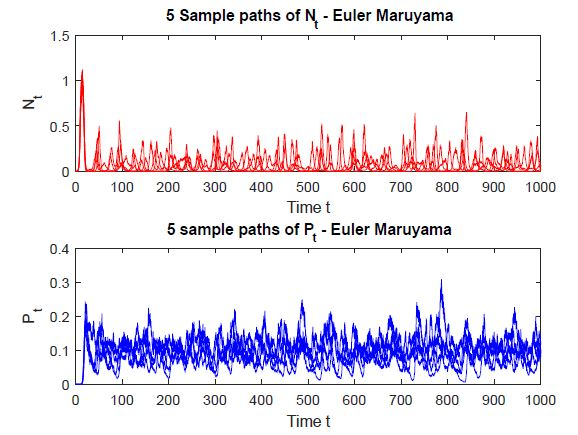
\includegraphics[height=9cm]{5simEM.JPG}
		\label{fig:23}
	\end{center}
\end{figure}
\FloatBarrier

Figure: 5 simulations of $N_t$ and $P_t$ up to time $T=1000$ with step size $h=10^{-3}$ in the Euler Maruyama scheme.\\

For $N_t$, we see something that could looks like stationary behavior from around time $100$. The population size seems to mostly be staying around $0~0.2$, and then making hikes up to around up to $0.3$, but larger hikes up to around $0.5$ also occur occasionally. $P_t$ seems to be staying around $0.1$ for the most of the time, but has also down and uptrips to around $0.05$ and $0.15$ mostly.


\begin{equation*}
\begin{aligned}

\end{aligned}
\end{equation*}


\FloatBarrier
\begin{figure}[ht]
	\begin{center}
		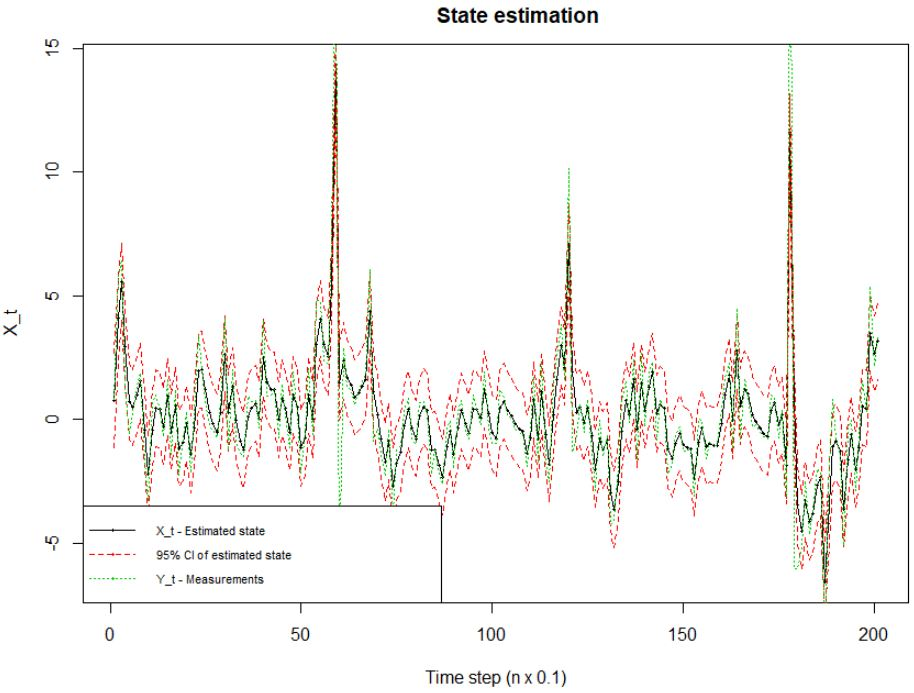
\includegraphics[height=10cm]{state_est.JPG}
		\label{fig:23}
	\end{center}
\end{figure}
\FloatBarrier


\[f(x,y)= \begin{cases} 
      \frac{2}{\pi} & (x,y)\in \Omega \\
      0  &\textrm{else}
   \end{cases}
\]



\section{Question 2 - A scalar mean-reverting process with state deependent noise intensity}



We have given the following It\^{o} process

\begin{equation}
\begin{aligned}
\label{ex21}
dX_t&=-\lambda X_t\cdot dt + \sigma\sqrt{1+X_t^2}\cdot dB_t
\end{aligned}
\end{equation}

with $B_t$ being a standard Brownian motion and $\sigma>0$\\

\subsection{Task 1 - The stationary distribution}

We do know want to determine the stationary distribution of the It\^{o} process in eq.~(\ref{ex21})


We have from Th. 9.4.1 in the notes that a the transition probabilites $\phi(t,y)$ for a given initial state $X_s=x$ is the probability density function for the state $X_t$ if the initial condition is random. Furthermore, this theorem states that since our stochastic process has the form Th. 9.1.1, then the density function of $X_t$ can found by solving the Forward Kolmogorov equation given by\\

\begin{equation*}
\begin{aligned}
\frac{\partial }{\partial t}\phi+\nabla (f\phi)-\nabla \bigcdot\nabla (D\phi)&=0
\end{aligned}
\end{equation*}

which for a our case, where $X_t$ takes values on $\mathbb{R}$ can be rewritten into advection-diffusion form



\begin{equation}
\begin{aligned}
\label{ex22}
\frac{\partial }{\partial t}\phi(t,x)&=-\frac{\partial}{\partial x}(u(x) \phi -D(x)\frac{\partial \phi}{\partial x})
\end{aligned}
\end{equation}

where $D(x)$ is the diffusity given by

\begin{equation*}
\begin{aligned}
D(x)&=\frac{1}{2}g(x)^2\\
&=\frac{1}{2}\sigma^2 (1+x^2)
\end{aligned}
\end{equation*}

and $u(x)=f(x)-D'(x)=-(\lambda + \sigma^2) x$ is the flow vector field.\\



In order to find the stationary distribution (steady state solution), we must solve eq.~(\ref{ex22}) for $\frac{\partial }{\partial t}\phi=0$\\


This gives us

\begin{equation*}
\begin{aligned}
0&=-\frac{\partial}{\partial x}(u(x) \phi -D(x)\frac{\partial \phi}{\partial x})\\
\end{aligned}
\end{equation*}

By integration with respect to $x$, we find

\begin{equation*}
\begin{aligned}
A&=(u(x) \phi -D(x)\frac{\partial \phi}{\partial x})\\
&=(-(\lambda+\sigma^2) x \phi -\frac{\sigma^2}{2} (1+x^2)\frac{\partial \phi}{\partial x})
\end{aligned}
\end{equation*}

Furthermore, our density for the stationary distribution must satisfy the no-flux condition, meaning that we find the homogeneous solution to the above differential equation, i.e. $A=0$\\


\begin{equation*}
\begin{aligned}
0&=(-(\lambda+\sigma^2) x \phi -\frac{\sigma^2}{2} (1+x^2)\frac{\partial \phi}{\partial x})
\end{aligned}
\end{equation*}

Since we now assume that $\phi$ is only a function of $x$, we write $\phi=\phi(x)$ and mark $\phi'$ as the derivative of $\phi$ wrt. x, we get the following ODE


\begin{equation*}
\begin{aligned}
\frac{\sigma^2}{2} (1+x^2)\cdot \phi'&=-(\lambda+\sigma^2) x\cdot \phi
\end{aligned}
\end{equation*}

Which has the solution given by\\

\begin{equation*}
\begin{aligned}
\phi(x)&=C\cdot e^{\int_{x_0}^x \frac{-2(\lambda+\sigma^2)x}{\sigma^2(1+x^2)} dx}
\end{aligned}
\end{equation*}

where $C$ is a normalization constant, such that $C=\frac{1}{\int_{-\infty}^{\infty} \phi(x)\cdot dx}$\\

We find the complete solution of $\phi$ to be ($x_0=0$ for convenience)


\begin{equation*}
\begin{aligned}
\phi(x)&=C\cdot e^{\int_{x_0}^x \frac{-2(\lambda+\sigma^2)x}{\sigma^2(1+x^2)} dx}\\
&=C\cdot e^{\int_{0}^x \frac{-2(\lambda+\sigma^2)x}{\sigma^2(1+x^2)}dx}\\
&=C\cdot e^{-\log(1+x^2)\cdot \frac{(\lambda+\sigma^2)}{\sigma^2}}\\
&=C\cdot (1+x^2)^{-\frac{(\lambda+\sigma^2)}{\sigma^2}}\\
\end{aligned}
\end{equation*}

We see that in order for $\phi(x)$ to be integrable, i.e. $\int_{-\infty}^{\infty} \phi(x) dx$ we must have that $-\frac{(\lambda+\sigma^2)}{\sigma^2}<-\frac{1}{2} \rightarrow 2\lambda>-\sigma^2$ must be fulfilled in order for $\phi(x)$ to be integrable.\\

Now, we normalize $(1+x^2)^{-\frac{(\lambda+\sigma^2)}{\sigma^2}}$ in order for $\phi(x)$ to integrate to $1$, so that it is a probability density\\


\begin{equation*}
\begin{aligned}
\frac{1}{C}&=\int_{-\infty}^{\infty} (1+x^2)^{-\frac{(\lambda+\sigma^2)}{\sigma^2}} dx\\
&=\frac{\sqrt{\pi}\cdot\Gamma(\frac{1}{2}+\frac{\lambda}{\sigma^2})}{\Gamma(1+\frac{\lambda}{\sigma^2})}
\end{aligned}
\end{equation*}

Hence we find the probability density for the stationary distribution to be



\begin{equation*}
\begin{aligned}
\phi(x)&=C\cdot (1+x^2)^{-\frac{(\lambda+\sigma^2)}{\sigma^2}}\\
&=\frac{\Gamma(1+\frac{\lambda}{\sigma^2})}{\sqrt{\pi}\cdot\Gamma(\frac{1}{2}+\frac{\lambda}{\sigma^2})}\cdot (1+x^2)^{-\frac{(\lambda+\sigma^2)}{\sigma^2}}
\end{aligned}
\end{equation*}

for $x\in \mathbb{R}$.\\

So to conclude, the condition for the existence of a stationary distributions is that we must chose our coefficient $(\lambda, \sigma)$ such that $2\lambda>-\sigma^2$.\\

Now we plot the stationary density for $\lambda=\sigma=1$.\\


Now, we look at the conditions for the stationary distribution to have finite mean and finite variance.\\

We start out with finite mean\\



\subsection{Task B - The dynamics of mean and variance}


We now fix our initial conditions $X_0=x$ and find analytical expressions for $\mathbb{E}[X_t]$ and $\mathbb{E}[X_t^2]$, starting with $\mathbb{E}[X_t]$\\

We start out with transforming the process $X_t$ into $Y_t=e^{-\lambda t}X_t$

\begin{equation*}
\begin{aligned}

\end{aligned}
\end{equation*}



\begin{equation*}
\begin{aligned}

\end{aligned}
\end{equation*}


\newpage
\begin{thebibliography}{99}


\bibitem{Test01} Uffe Høgsbro Thygesen - Lecture Notes on Diffusion and Stochastic Differential Equations, August 19, 2016



\end{thebibliography}


\end{document}
